\setlength{\headheight}{15pt}
\addtolength{\topmargin}{-2.5pt}

\chapter{Technology Review}

\section{Executive Dashboard}
When it came to developing the Executive Dashboard for data analysis it was crucial to select the tools that could transform data into easily comprehensible information. After conducting research and exploring alternatives Angular and Chart.js were chosen for specific reasons.

\subsection{Angular}
Angular is based on TypeScript and is an open-source framework, and it's a great tool for building client-side web applications. It can be used for single-page applications (SPAs) or for enterprise-level solutions.

\subsubsection{Main Concepts: Components, Modules and Services}
Angular is composed of three foundational blocks: Components, Modules and services.

\subsubsection{Components} Components are like Lego blocks of the application. Each component holds a portion of the user interface and its behaviour. Components serve as the bridge between the application data and what the user experiences on the screen.\cite{angular-components}

\subsubsection{Modules} In Angular modules serve as containers that group related components, directives, and services together that can be combined with other modules. It plays an important role in improving maintainability and re-usability, key concepts of Angular development.\cite{angular-modules}

\subsubsection{Services} Angular services use typescript classes with injectable decorators. The decorator tells angular that the class is a service and can be injected into other components that need that service.\cite{angular-services}


\subsection{Angular architecture}
Angular uses the Model-View-Controller (MVC) pattern, with a variation known as Model-View-ViewModel (MVVM). The controller is responsible for the interaction between the model and the view.

\begin{figure}[ht]
    \centering
    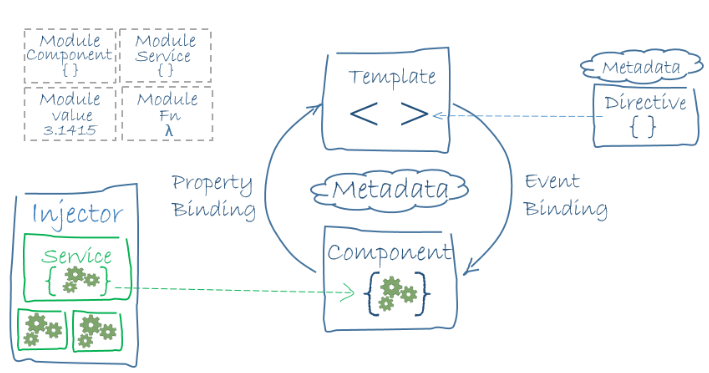
\includegraphics[width=0.85\linewidth]{images/angular-arch.png}
    \caption{Angular application architecture}
    \label{fig:angular-arch}
\end{figure}

\subsection{Advantages of using Angular}
\subsubsection{Component-Based Architecture}
As mentioned earlier in discussions Angular organisess its functionalities into components. These components have the ability to communicate with each other enabling updates to sections without affecting the rest of the application.

\subsubsection{Mobile-Friendly Approach}
Angular incorporates techniques such, as lazy-loading, which means loading parts of the application (like images) only when they are needed. This ensures that users do not experience long waiting times.

\subsubsection{Two-Way Data Binding}
With Angular two way data binding data can seamlessly flow between the component and the view allowing for synchronization.

\subsubsection{Asynchronous Programming}
By utilizing programming executes code in a non-sequential manner and employs multi-threading to enhance performance. This speeds up operations and prevents system freezes, providing users with a seamless experience.

\subsubsection{Single-Page Applications}
Angular creates a dynamic single-page application which can be navigated without page reloads, improving the user experience with better user interaction and engagement.

\subsubsection {Code Re-usability}
The component-based architecture of Angular promotes the re-usability of UI components saving development time.

\subsubsection{Dependency Injection}
With dependency injection in place, Angular allows for the creation of objects that rely on other objects. This improves modularity and efficiency, within the app.

\subsubsection{Angular Material}
Angular's documentation offers a range of built user interface components and modules that adhere to Google's Material Design principles. This greatly facilitates the developer's work, simplifying the design process and enabling application development.

\subsubsection{Angular CLI} Angular command line interface gives the developer the ability to generate Angular projects, modules, services, and components with a single command, this not only saves time but also reduces configuration errors, it gives the developer the freedom to dive into creative aspects of the project, focusing on innovation and functionality rather than getting bogged down by initial setup complexities.

Angular command line interface gives the developer the ability to generate Angular projects, modules, services, and components with a single command, this not only saves time but also reduces configuration errors, it gives the developer the freedom to dive into creative aspects of the project, focusing on innovation and functionality rather than getting bogged down by initial setup complexities.

\section{Data Visualization}

Data visualization is the process of translating large volumes of data into visual representations. It is a powerful tool that allows for the identification of patterns and trends that would otherwise be difficult to identify. It is a key component of data analysis and is used to communicate information clearly and efficiently.

\subsection{Chart.js}
Chart.js is robust, lightweight and open source javascript library that provides features for creating visually appealing charts and graphs that can be embedded into a web page. It is a great tool for data visualization and is easy to use. It is based on HTML5 canvas and is responsive, meaning that the charts will adapt to the size of the container element. It is also compatible with all modern browsers and is supported by a large community of developers. \cite{da2019learn}
It can be compared like a the artist's toolkit for developers, providing a flexible API to create a variety of chart types, such as line charts, radar charts, pie charts and many more. It also provides a range of customization options, allowing developers to create unique and visually appealing charts. \cite{da2019learn}

Table \ref{tab:chart-js-features} is showing some of the features of Chart.js\cite{da2019learn}:

\begin{table}[H]
    \centering

    \begin{tabularx}{\textwidth}{|l|X|}
        \hline
        \textbf{Feature}            & \textbf{Description}                                                                                                                                                                                                \\
        \hline
        Easy to use                 & Aesthetically charts can be created without the need of extensive configuration. The library follows a declarative approach allowing the developer to define the data and settings of the chart in a single object. \\
        \hline
        Responsive                  & Charts generated by Chart.js are responsive, adapting to different screen sizes and devices, ensuring that the visualization remains accessible and readable across various platforms.                              \\
        \hline
        Customization               & Chart.js provides a high degree of customization. Colors, fonts, and other visual elements can be customized to create unique and visually appealing charts.                                                        \\
        \hline
        Interactivity               & Chart.js provides built-in support for tooltips and animation, allowing the user to explore data points, adding a layer of engagement to the project.                                                               \\
        \hline
        Cross-browser compatibility & Chart.js is compatible with all modern browsers, including Chrome, Firefox, Safari, Edge, and Internet Explorer 11.                                                                                                 \\
        \hline
    \end{tabularx}
    \label{tab:chart-js-features}
    \caption{Chart.js Features}
\end{table}


Chart.js is a reliable and effective tool for data visualization, it is also easy to use and provides a range of customization options. It is also supported by a large community of developers, which is a great advantage.

\subsection{D3.js}
D3.js or Data-Driven Documents is a JavaScript library for manipulating documents based on data. It has the ability ti bind data to the DOM (Document Obect Model) and creates interactive and dynamic visualization. It provides a lower level and more granular approach to data visualization, giving the developer more control over the visualization process.\cite{d3}


Table \ref{tab:d3-js-features} is showing some of the features of D3.js\cite{d3}:

\begin{table}[H]
    \centering

    \begin{tabularx}{\textwidth}{|l|X|}
        \hline
        \textbf{Feature} & \textbf{Description}                                                                                                                                                      \\
        \hline
        Data-Driven      & D3.js is data-driven, meaning that it can bind data directly to HTML or SVG elements. This type of control is advantageous for creating highly customized visualizations. \\
        \hline
        Modular          & D3.js is modular, composed of many small modules that can be used independently or combined together to create a custom visualization.                                    \\
        \hline
        Extensible       & D3.js is extensible, meaning that it can be extended to support any type of visualization.                                                                                \\
        \hline
        Community        & D3.js is supported by a large community of developers, which is a great advantage.                                                                                        \\
        \hline
    \end{tabularx}
    \label{tab:d3-js-features}
    \caption{D3.js Features}
\end{table}


D3.js is a powerful tool for data visualization, it provides a high degree of customization and control over the visualization process. However, it is more complex and requires more time to learn and implement. It is also not supported by all browsers, which is a disadvantage.

In conclusion, while D3.js is a powerful tool for data visualization, it is more complex and requires more time to learn and implement. It is also not supported by all browsers, which is a disadvantage. Considering the scope of the project and the time constraints, Chart.js was chosen as the tool for data visualization. It is easy to use and provides a high degree of customization, allowing for the creation of unique and visually appealing charts. It is also supported by a large community of developers, which is a great advantage.

\section{AI module - Data analysis}
Ninety per cent of the world's data was generated in just the last two years. In the early 2000s, the amount of data being generated exploded exponentially with the use of the internet, social media, and various other technologies. Organizations found themselves facing a massive volume of data that was very hard to process. To address the challenge, the concept of Big data emerged. Big data refers to extremely large and complex data sets that are difficult to process using traditional methods. \cite{bigdata}

\subsection{Hadoop}
As the volume of data grew rapidly across the globe, organizations needed a way to manage it to gain valuable insights. That’s where Hadoop came in. In 2006, a team of engineers from Yahoo developed Hadoop inspired by Google’s MapReduce. Hadoop has introduced a new way of handling data called distributed processing. Now, to process all data it wouldn't use single machines anymore, instead, Hadoop uses multiple computers, allowing large amounts of data to be processed way faster than before.
Hadoop has mainly two main components: HDFS (Hadoop Distributed File System) and MapReduce. HDFS stores the into multiple computers, and MapReduce is responsible for processing the data in parallel allowing the organizations to store and process large amounts of data.
Hadoop was a great advance in big data processing, however, it had a few limitations. One of the biggest problems was that it relied on storing data on disk. This slowed down data processing because every time a job ran it had to save its data to disk, read it back, process it, and save it back to disk Another problem is that Hadoop processes data only in batches. This means a new job couldn't be submitted before the other job ended.
With Hadoop, storing and processing large amounts of data became possible, even with some limitations it was an important step in big data processing.\cite{hadoop}


\subsection{Apache Spark}
As described Hadoop has a few limitations, there was a need to process all this data faster and in real-time. And here is where Apache Spark comes into action. In 2009, researchers at the University of California developed Apache Spark as a research project. At this point, RDD (Resilient Distributed Dataset) was introduced and deemed to be a very powerful concept.\cite{apache-spark}
RDD is the backbone of Apache Spark, storing the data in memory for faster access and processing. It will not read and write the data from the disk, instead, Spark processes the entire data just in memory. The meaning of memory here is the RAM (Random Access Memory) stored inside the computer. This in-memory data processing of data makes Spark much faster than Hadoop.
Spark also gives the ability to write code in various programming languages such as JAVA, Scala, Python and R, along with an optimized engine that supports general execution graphs.

\subsubsection{Main components and Features}

\begin{figure}[ht]
    \centering
    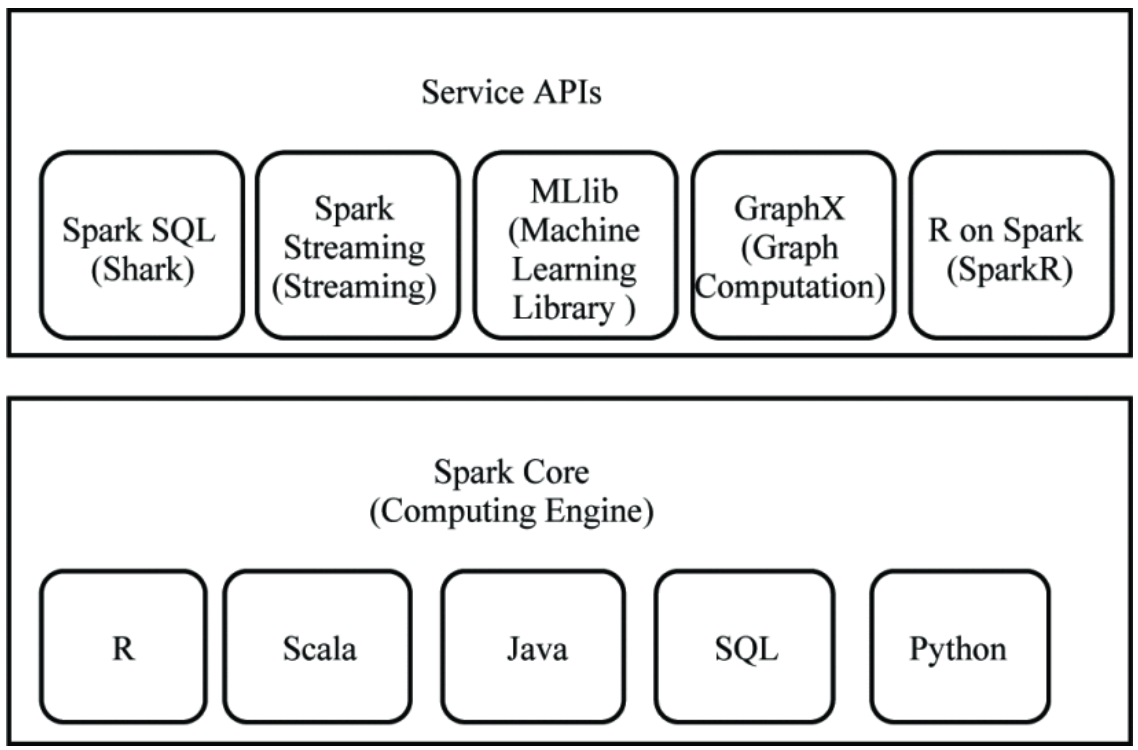
\includegraphics[width=1\linewidth]{images/Spark_Eco.png}
    \caption{Apache Spark Ecosystem}
    \label{fig:spark-eco}
\end{figure}

The Apache Spark ecosystem consists of the following main components\cite{8988541}:
\begin{itemize}
    \item Spark SQL: Formerly known as Shark.  Spark SQL is a distributed framework that works with structured and semi-structured data. It facilitates analytical and interactive applications for both streaming and historical data which can be accessed from various sources such as JSON, Parquet and Hive table.\cite{8988541}
    \item Spark Streaming: Allows to process real-time data. Is a scalable fault-tolerant streaming processing system that supports both batch and streaming workloads. Spark streaming enhances the fast scheduling capability of Apache Spark by inserting data into mini-batches. An operation known as transformation is then applied to those mini-batches that can be easily obtained from live streams and data sources such as Twitter, Apache Kafka, IoT sensors, and Amazon Kinesis.\cite{8988541}
    \item Spark Core: One of the most important parts of the Spark ecosystem is called Spark Core. It helps process data across multiple computers and ensures everything works efficiently and smoothly. Various functionalities of Apache Spark are built on top of the Spark core. It provides a vast range of APIs as well as applications for programming languages such as Scala, Java, and Python APIs to facilitate the ease of development. In-memory computation is implemented in Spark core in order to deliver speed and solve the issue of MapReduce.

    \item MLlib: It delivers high-quality algorithms with high speed and makes machine learning easy to use and scale. Several machine learning algorithms such as regression, classification, clustering, and linear algebra are present. It also provides a library for lower-level machine learning primitives like the generic gradient descent optimization algorithm. It also provides other functions such as model evaluation and data import. It can be used in Java, Scala, and Python. \cite{8988541}
\end{itemize}

With all these components working together, Apache Spark became a powerful tool for processing and analysing Big Data. Spark manages and coordinates the execution of tasks on data across a cluster of computers.

\begin{figure}[H]
    \centering
    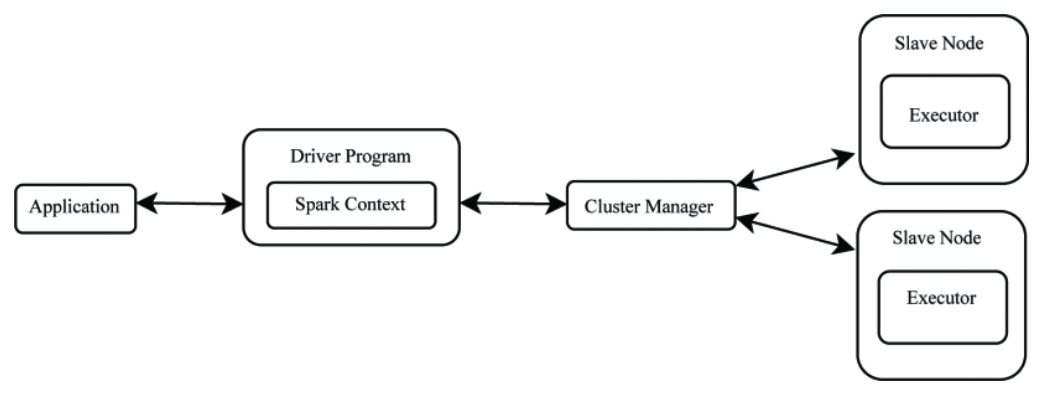
\includegraphics[width=1\linewidth]{images/Spark_Arch.png}
    \caption{Apache Spark Architecture}
    \label{fig:spark-arch}
\end{figure}

Figure~\ref{fig:spark-arch} shows the Spark Architecture. It consists of a master node which has a driver program that is responsible for calling the main program of an application, this driver could be the Spark shell or the application, written in Scala or Java, for example. It is basically the entry point and is responsible for creating Spark context, which behaves like a gateway to all of the functionalities of Apache Spark. It allows for communication and coordination with other nodes within the cluster, known as Slave nodes. Within the slave node, there are many numbers of executors which act as workers. Whenever a job is initiated, the driver process will make sure it goes through the Apache application properly. It analyzes the work that needs to be done, divides it into smaller tasks and assigns it to the executors. The driver process is the heart of the Apache Spark application and executors are the real workers, which execute the work assigned by the driver and report back the progress and results of the computation.\cite{8988541}

Due to the powerful capabilities of distributed computing, large volumes of data can be processed quickly and efficiently. For all these reasons, it was deemed to be the perfect technology to be used in this project. As the project evolves and more data is gathered from our research volunteers, Spark's performance scales with the size of the data, processing with high speed.


\subsection{Node JS}
NodeJS is an open-source, cross-platform, JavaScript runtime environment that executes JavaScript code outside of a browser. It is built on Chrome's V8 JavaScript engine and is used to build fast and scalable network applications. It is event-driven and non-blocking, meaning that it is capable of handling concurrent operations without blocking the execution of other operations. This makes it ideal for data-intensive real-time applications that run across distributed devices.\cite{nodejs}
It has solidified its position as a cornerstone of modern web development, with a large community of developers and a vast ecosystem of open-source libraries.

\subsubsection*{Advantages of Node.js}
It is an asynchronous event-driven JavaScript runtime environment that is designed to build scalable network applications. It is lightweight and efficient, making it a great choice for data-intensive real-time applications.\cite{tilkov}
One of the primary advantages of NodeJS is that it uses a single-threaded event loop, which allows it to handle concurrent operations without blocking the execution of other operations.
Another strength of NodeJS is its vast ecosystem of open-source libraries. The Node Package Manager (NPM) is the largest ecosystem of open-source libraries in the world, with over 1 million packages. \cite{npm} This
wealthy of modules and libraries greatly facilitates the development process, allowing developers to focus on the creative aspects of the project, rather than reinventing the wheel.
NodeJS also benefits from its single programming language across both the server and client sides. This allows for the sharing of code and data between the server and the client, which is a great advantage, reducing the learning curve associated with NodeJS development. \cite{tilkov}
Performance wise NodeJS is very fast, it is built on Chrome's V8 JavaScript engine, which is a high-performance JavaScript engine. It is also lightweight and efficient, making it a great choice for data-intensive real-time applications. \cite{tilkov}

\subsubsection*{Disadvantages of Node.js}
NodeJS is not without its criticisms. Critics often point out the callback hell, a situation where the code becomes unreadable due to the excessive use of callbacks. Although it has been largely mitigated by the introduction of Promisses and async/await syntax, it remanins a valid criticism. \cite{cantelon2014node}

Table \ref{tab:node-js-advantages-disadvantages} is summarizing the advantages and disadvantages of Node.js\cite{tilkov}:

\begin{table}[H]
    \centering
    \begin{tabularx}{\textwidth}{|X|X|}
        \hline
        \textbf{Advantages of Node.js}                                                                                                               & \textbf{Disadvantages of Node.js}                                                                                                                              \\
        \hline
        Non-blocking and event-driven: Allows for high concurrency and scalability, making it suitable for real-time applications.                   & Single-threaded: Node.js is single-threaded, which can lead to blocking if not handled correctly, impacting CPU-bound tasks.                                   \\
        \hline
        JavaScript as a single language: Developers can use JavaScript for both server-side and client-side development, reducing context switching. & Callback hell: Deeply nested callbacks can make the code hard to read and maintain (though Promises and async/await mitigate this issue).                      \\
        \hline
        Large and active community: A vast number of open-source libraries and modules available through npm (Node Package Manager).                 & Limited support for multi-core processors: Node.js does not fully utilize multi-core CPUs out of the box.                                                      \\
        \hline
        Speed: Node.js is built on the V8 JavaScript engine, known for its high-performance execution.                                               & Less suitable for CPU-intensive tasks: Due to its event-driven, single-threaded nature, Node.js may not be the best choice for CPU-bound operations.           \\
        \hline
        Lightweight and fast startup: Node.js applications typically have lower memory consumption and quicker startup times.                        & Maturity and stability: Some developers argue that Node.js, compared to more established platforms, may have less maturity and stability in certain use cases. \\
        \hline
    \end{tabularx}
    \label{tab:node-js-advantages-disadvantages}
    \caption{Advantages and Disadvantages of Node.js}
\end{table}


Considering these noumerous advantages, NodeJS was chosen as the technology for the project. It is lightweight and efficient, making it a great choice for data-intensive real-time applications. It also benefits from its vast ecosystem of open-source libraries, which greatly facilitates the development process, allowing us to focus on the creative aspects of the project, rather than reinventing the wheel. It is also fast and scalable, which is a great advantage.


\subsection{PM2}
PM2, or Process Manager 2, is a production process manager for NodeJS applications. It is a feature-rich tool that provides a wide range of features, including monitoring, load balancing, and error handling. It is designed to simplify the deployment and management of NodeJS applications in production environments and to keep applications alive forever, restart
them without downtime and simplify common system administration tasks.
The standout feature of PM2 is its ability to keep processes running in the background indefinitely. This is particular important for web applications that requires constant availability. PM2 automatically resurrects crashed applications, ensuring that system glitches do not result in prolonged downtime.\cite{pm2}
This automatic restart capability is a safeguard against potentially costly application crashes that could otherwise lead to a poor user experience or even lost revenue. \cite{pm2}
PM2 also provides a built-in load balancer that can distribute incoming requests across multiple instances of the application. This improves performance and scalability, allowing the application to handle more requests, evenly distributing traffic across the instances, which can be particularly beneficial when running on multi-core systems. \cite{pm2LoadBalancing}
However, PM2 is not one-size-fits-all solution. It is designed for NodeJS applications, and is not suitable for applications written in other languages. It is also not suitable for applications that require a high degree of customization. \cite{pm2}
Despite the considerations, PM2's benefits have outweighed its limitations, and it was chosen as the technology for the project. It is a feature-rich tool that provides a wide range of features, including monitoring, load balancing, and error handling.
It is designed to simplify the deployment and management of NodeJS applications in production environments and to keep applications alive forever, restart them without downtime and simplify common system administration tasks.
Its installation and setup process is straightforward, requiring minimal configuration. It is also lightweight and efficient, making it a great choice for this project. \cite{tilkov}

\subsection{Docker}

Docker has emerged as a revolutionary tool for software development. It is an open-source platform that allows developers to build, ship, and run applications in containers. It is a lightweight alternative to virtual machines, allowing for the isolation of applications and their dependencies into containers. Containers encapsulate the application's code, libraries, and dependencies in a single object, ensuring that the application runs reliably and consistently across different environments.
Due to its simplicity and portability, Docker has become the de facto standard for containerization. It is supported by all major cloud providers, including Amazon Web Services, Microsoft Azure, and Google Cloud Platform. Its lightweight nature compared to traditional virtual machines makes it ideal for cloud computing. Containers share the machine's OS kernel, and do not require an OS per application, which greatly reduces the memory footprint and improves performance. \cite{merkel2014docker}

\begin{figure}[ht]
    \centering
    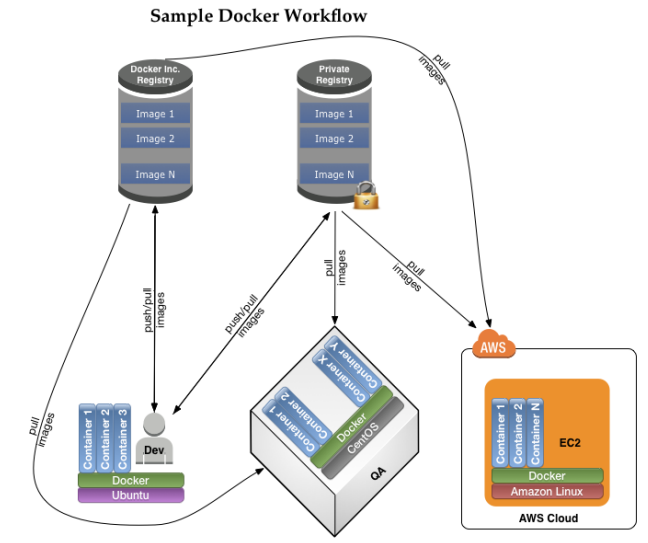
\includegraphics[width=0.8\linewidth]{images/docker.png}
    \caption{Development workflow with Docker}
    \label{fig:docker}
\end{figure}

However, Docker's container model is not without challenges. In the context of this project, the average size of a single Docker image exceeding 400MB presents a concern regarding bandwidth utilization. Continous build and deployment processes involving large container images can consume substantial network resources, leading to potential cost overruns. \cite{merkel2014docker}
Another challenge is the security of Docker containers. Docker containers share the same kernel, which means that a vulnerability in the kernel can affect all containers. \cite{dockerhub}
While Docker's layering and image caching mechanisms can mitigate some of the network overhead, it is still a concern.
In conclusion, Docker is a powerful tool that offers numerous benefits for application deployment, from development to production. However, it is not without its challenges. The large size of Docker images can lead to bandwidth utilization issues, and the shared kernel model can lead to security concerns. Considering the scope of the project, time constraints and budget, Docker wasn't chosen as the technology for the project as the cost would be too high.


\subsection{NGINX}
NGINX is a high-performance web server that can also be used as a reverse proxy, load balancer, mail proxy, and HTTP cache. It is a lightweight and efficient solution that can handle high volumes of concurrent connections. It is also highly configurable, allowing for the customization of its behaviour to suit the needs of the application.
It was originally created by Igor Sysoev in 2004, with the goal of solving the C10K problem, which refers to the challenge of handling 10,000 concurrent connections. \cite{nginx} It has since become one of the most widely used web servers in the world, often used as load balancer and as reverse proxy in addition to its role as a web server.

Table \ref{tab:ngnix} is showing some of the features of NGINX\cite{nginx}:

\begin{table}[H]
    \centering
    \begin{tabularx}{\textwidth}{|l|X|}
        \hline
        \textbf{Aspect}        & \textbf{Description}                                                                                                                      \\
        \hline
        Type                   & Web server software                                                                                                                       \\
        \hline
        Primary Use            & Serving web content, load balancing, reverse proxy, and more                                                                              \\
        \hline
        Performance            & Highly efficient in handling high concurrency with low memory footprint                                                                   \\
        \hline
        Architecture           & Event-driven, asynchronous, and non-blocking which contributes to its ability to handle a large number of simultaneous connections easily \\
        \hline
        Scalability            & Scalable to support growth in traffic and applications                                                                                    \\
        \hline
        Security Features      & Offers robust security features including rate limiting, client request filtering, and SSL/TLS termination                                \\
        \hline
        Flexibility            & Highly configurable for a wide range of web and mail server tasks                                                                         \\
        \hline
        Open Source/Commercial & Available in both open-source and commercial versions (NGINX Plus)                                                                        \\
        \hline
    \end{tabularx}
    \label{tab:ngnix}
    \caption{NGINX Features}
\end{table}

Due to its vast capabilities NGNIX was chosen for our project as reverse proxy and load balancer. It is a lightweight and efficient solution that can handle high volumes of concurrent connections. It is also highly configurable, allowing for the customization of its behaviour to suit the needs of the application.

\subsection{MySQL}
MySQL is an open-source relational database management system (RDBMS) that is widely used in web applications. It uses structured query language (SQL) for database access and is known for its speed, reliability, and ease of use. MySQL is a popular choice for both small and large applications and is an essential component of the LAMP (Linux, Apache, MySQL, PHP/Perl/Python) software stack.

Table \ref{tab:mysql} is showing some of the features of MySQL\cite{mysql}:

\begin{table}[H]
    \centering
    \begin{tabularx}{\textwidth}{|l|X|}
        \hline
        \textbf{Aspect}          & \textbf{Description}                                                                                                   \\
        \hline
        Data Handling            & Efficiently manages large datasets, crucial for training machine learning models                                       \\
        \hline
        Query Performance        & Fast query execution, beneficial for data retrieval and preprocessing in machine learning workflows                    \\
        \hline
        Scalability              & Easily scales with data volume and complexity, supporting the growing needs of machine learning applications           \\
        \hline
        ACID Compliance          & Ensures data integrity and consistency, vital for the accuracy of machine learning outputs                             \\
        \hline
        Advanced Analytics       & Supports SQL extensions for advanced analytics, facilitating machine learning data processing tasks                    \\
        \hline
        Data Storage Options     & Offers various storage engines, allowing optimization based on the specific needs of machine learning models           \\
        \hline
        Community and Support    & Strong community and extensive documentation, aiding in troubleshooting and optimization for machine learning projects \\
        \hline
        Integration Capabilities & Easily integrates with popular machine learning frameworks and languages, streamlining the development process         \\
        \hline
    \end{tabularx}
    \label{tab:mysql}
    \caption{MySQL}
\end{table}

In the context of this project, the dataset was originally in a JSON format in FireStore which were found to be of a high complexity while performing compound querying. To facilitate querying and the high complexities involved in FireStore,
MySQL was chosen to be the database for the project, where all the data for analysis is sourced directly from it, which is a structured replica of the FireStore Database as obtained from the Legacy System.\\
By regularizing the data in MySQL, a more standardized and organized dataset was achieved. This standardization significantly simplified the data preprocessing steps in the machine learning workflow.


\subsection{Express JS}
Express.js, commonly referred as Express, is a minimal and flexible Node.js web application framework that provides a robust set of features for web and mobile applications. It is widely used for building server-side applications and APIs due to its simplicity, performance, and scalability. In this project, Express.js was chosen for several strategic reasons, which are outlined below.\cite{express}

\begin{table}[H]
    \centering
    \begin{tabularx}{\textwidth}{|l|X|}
        \hline
        \textbf{Feature}     & \textbf{Advantage for Our Project}                                                                                                                              \\
        \hline
        Minimalist Framework & Express.js provides essential web application features without dictating any specific architecture, allowing for flexibility and customization in our project.  \\
        \hline
        Middleware Support   & The use of middleware modules enables us to extend the functionality of our application easily and efficiently.                                                 \\
        \hline
        Routing System       & Its powerful routing system helps manage requests and responses effectively, a crucial aspect for our project's RESTful API design.                             \\
        \hline
        High Performance     & Known for its high performance, Express.js enhances the responsiveness and speed of our web application.                                                        \\
        \hline
        Community Support    & Being one of the most popular Node.js frameworks, it has strong community support, ensuring access to a wide range of resources and troubleshooting assistance. \\
        \hline
        Easy Integration     & Express.js seamlessly integrates with other technologies and databases, which is vital for the diverse tech stack of our project.                               \\
        \hline
        Simplicity           & Its simplicity and ease of use accelerate development and reduce the learning curve for new team members.                                                       \\
        \hline
    \end{tabularx}
    \label{tab:expressJS}
    \caption{Express.js Features}
\end{table}

It was chose as a back end web application for this project due to its simplicity, performance, and scalability. It is also widely used for building server-side applications and APIs, which is a great advantage. It also provides a robust set of features for web and mobile applications, which is a great advantage.

\subsection{TensorFlow}


